\documentclass[aspectratio=169]{beamer}
\usepackage{tikz}
\usepackage{graphicx}
\usetikzlibrary{shapes.geometric, arrows, positioning, decorations.pathmorphing}

% Define simple icon commands as text substitutes
\newcommand{\faLock}{$\bigstar$}
\newcommand{\faSmile}{$\smile$}
\newcommand{\faRocket}{$\Rightarrow$}
\newcommand{\faTelegramPlane}{$\triangleright$}
\newcommand{\faRobot}{$\square$}
\newcommand{\faImage}{$\diamondsuit$}
\newcommand{\faCoins}{$\circ$}
\newcommand{\faTwitter}{$\star$}
\newcommand{\faParachuteBox}{$\clubsuit$}
\newcommand{\faBook}{$\parallel$}
\newcommand{\faPenFancy}{$\sim$}
\newcommand{\faCode}{$\{ \}$}
\newcommand{\faCheckCircle}{$\checkmark$}
\newcommand{\faShieldAlt}{$\triangle$}
\newcommand{\faChartLine}{$\nearrow$}
\newcommand{\faCrown}{$\spadesuit$}
\newcommand{\faCog}{$\otimes$}
\newcommand{\faMusic}{$\sharp$}
\newcommand{\faCat}{$\heartsuit$}
\newcommand{\faUsers}{$\odot$}

% Custom theme with punk rock cute aesthetic
\usetheme{Madrid}
\usecolortheme{rose}

% Define custom colors - demure punk rock cute palette
\definecolor{punkpink}{RGB}{255,182,193}
\definecolor{darkpunk}{RGB}{51,51,51}
\definecolor{cuteviolet}{RGB}{186,85,211}
\definecolor{rebelred}{RGB}{220,20,60}
\definecolor{softblack}{RGB}{40,40,40}

\setbeamercolor{background canvas}{bg=white}
\setbeamercolor{frametitle}{fg=darkpunk,bg=punkpink}
\setbeamercolor{title}{fg=rebelred}
\setbeamercolor{structure}{fg=cuteviolet}
\setbeamercolor{normal text}{fg=softblack}
\setbeamercolor{item}{fg=rebelred}

% Remove navigation symbols
\setbeamertemplate{navigation symbols}{}

% Custom title page
\setbeamertemplate{title page}[default][colsep=-4bp,rounded=true]

% Fonts
\setbeamerfont{title}{size=\Huge,series=\bfseries}
\setbeamerfont{subtitle}{size=\Large}
\setbeamerfont{frametitle}{size=\large,series=\bfseries}

\title{\textcolor{rebelred}{Foid.Fun}}
\subtitle{\textcolor{cuteviolet}{Privacy Launchpad}}
\author{}
\date{}

\begin{document}

% Slide 1: Title Slide
\begin{frame}[plain]
\begin{center}
\vspace{2cm}
{\Huge\textbf{\textcolor{rebelred}{Foid.Fun}}}
\vspace{1cm}

{\Large\textcolor{cuteviolet}{Privacy Launchpad}}
\end{center}
\end{frame}

% Slide 2: Privacy & Memes Together
\begin{frame}
\frametitle{Privacy \& Memes Together}
\vspace{1cm}
\begin{center}
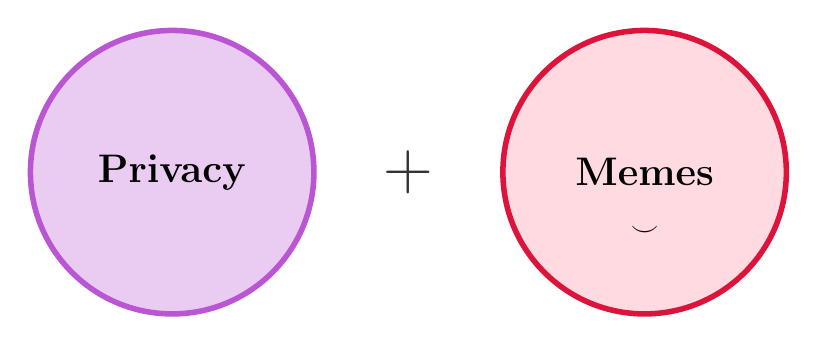
\begin{tikzpicture}[scale=1.5]
% Privacy circle
\draw[fill=cuteviolet!30, draw=cuteviolet, line width=2pt] (-2,0) circle (1.2cm);
\node at (-2,0) {\Large\textbf{Privacy}};
\node at (-2,-0.5) {\faLock};

% Memes circle
\draw[fill=punkpink!50, draw=rebelred, line width=2pt] (2,0) circle (1.2cm);
\node at (2,0) {\Large\textbf{Memes}};
\node at (2,-0.5) {\faSmile};

% Plus sign
\node at (0,0) {\Huge\textcolor{darkpunk}{+}};
\end{tikzpicture}
\end{center}
\end{frame}

% Slide 3: Playground for Privacy Primitives
\begin{frame}
\frametitle{Playground for Privacy Primitives}
\vspace{0.5cm}
\begin{center}
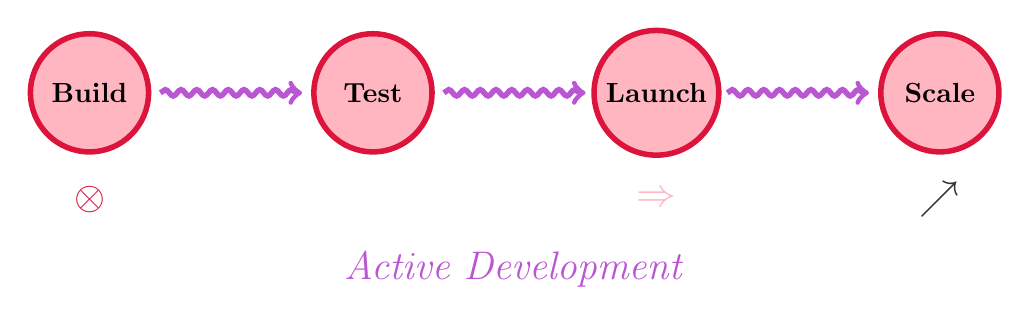
\begin{tikzpicture}[scale=0.9]
% Activity nodes
\foreach \x/\label in {0/Build, 4/Test, 8/Launch, 12/Scale} {
    \node[circle, fill=punkpink, draw=rebelred, line width=2pt, minimum size=1.5cm] at (\x,2) {\textbf{\label}};
}

% Connecting arrows with decorations (shorter arrows with more padding)
\draw[->, line width=2pt, cuteviolet, decorate, decoration={snake, amplitude=.4mm, segment length=2mm}] (1,2) -- (3,2);
\draw[->, line width=2pt, cuteviolet, decorate, decoration={snake, amplitude=.4mm, segment length=2mm}] (5,2) -- (7,2);
\draw[->, line width=2pt, cuteviolet, decorate, decoration={snake, amplitude=.4mm, segment length=2mm}] (9,2) -- (11,2);

% Activity indicators below with unique icons
\node at (0,0.5) {\Large\textcolor{rebelred}{\faCog}}; % Build
\node at (4,0.5) {\Large\textcolor{cuteviolet}{\faCheckCircle}}; % Test
\node at (8,0.5) {\Large\textcolor{punkpink}{\faRocket}}; % Launch
\node at (12,0.5) {\Large\textcolor{darkpunk}{\faChartLine}}; % Scale

\node at (6,-0.5) {\Large\textcolor{cuteviolet}{\textit{Active Development}}};
\end{tikzpicture}
\end{center}
\end{frame}

% Slide 4: Ground Zero for Privacy PMF
\begin{frame}
\frametitle{Ground Zero for Privacy PMF}
\vspace{0.5cm}
\begin{center}
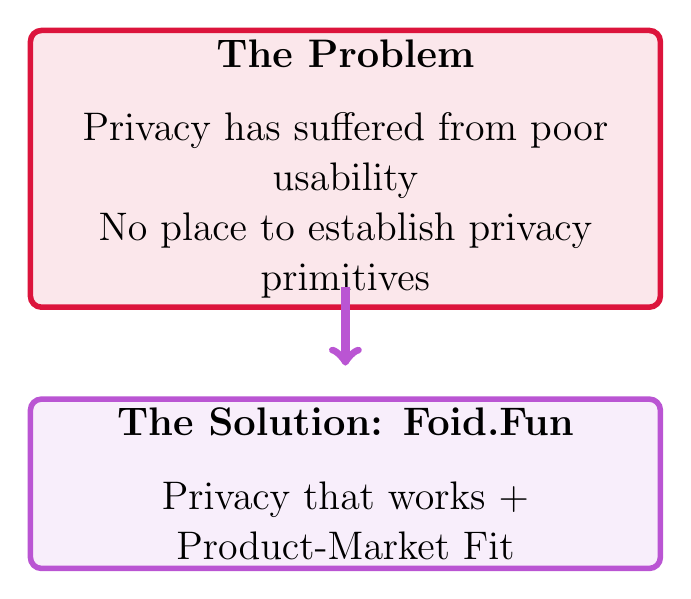
\begin{tikzpicture}
% Problem box
\node[rectangle, draw=rebelred, fill=rebelred!10, line width=2pt, minimum width=8cm, minimum height=2cm, rounded corners] at (0,2) {
    \begin{minipage}{7cm}
    \centering
    \Large\textbf{The Problem}\\[0.3cm]
    Privacy has suffered from poor usability\\
    No place to establish privacy primitives
    \end{minipage}
};

% Arrow
\draw[->, line width=3pt, cuteviolet] (0,0.5) -- (0,-0.5);

% Solution box
\node[rectangle, draw=cuteviolet, fill=cuteviolet!10, line width=2pt, minimum width=8cm, minimum height=2cm, rounded corners] at (0,-2) {
    \begin{minipage}{7cm}
    \centering
    \Large\textbf{The Solution: Foid.Fun}\\[0.3cm]
    Privacy that works + Product-Market Fit
    \end{minipage}
};
\end{tikzpicture}
\end{center}
\end{frame}

% Slide 5: Fluent in Privacy and Memes
\begin{frame}
\frametitle{Fluent in Privacy and Memes}
\vspace{0.5cm}
\begin{center}
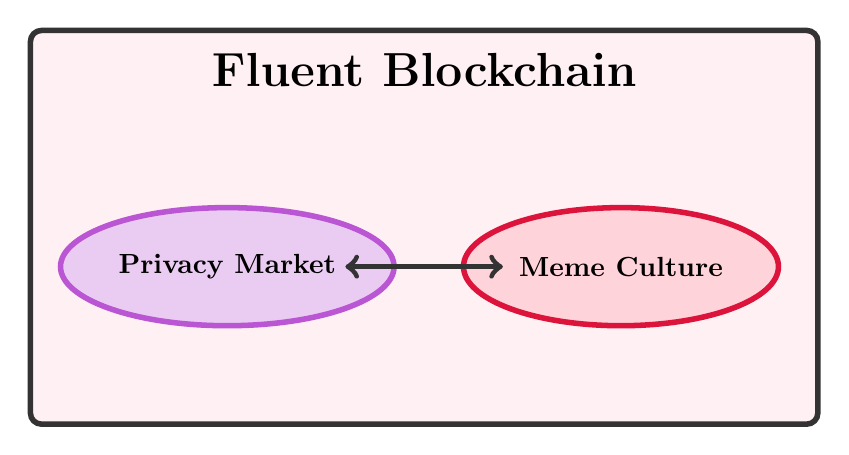
\begin{tikzpicture}
% Fluent blockchain background
\node[rectangle, draw=darkpunk, fill=punkpink!20, line width=2pt, minimum width=10cm, minimum height=5cm, rounded corners] at (0,0) {};
\node at (0,2) {\LARGE\textbf{Fluent Blockchain}};

% Privacy market
\node[ellipse, fill=cuteviolet!30, draw=cuteviolet, line width=2pt, minimum width=4cm, minimum height=1.5cm] at (-2.5,-0.5) {
    \textbf{Privacy Market}
};

% Meme culture
\node[ellipse, fill=punkpink!60, draw=rebelred, line width=2pt, minimum width=4cm, minimum height=1.5cm] at (2.5,-0.5) {
    \textbf{Meme Culture}
};

% Connection
\draw[<->, line width=2pt, darkpunk] (-1,-0.5) -- (1,-0.5);
\end{tikzpicture}
\end{center}
\end{frame}

% Slide 6: Apps Live on Testnet
\begin{frame}
\frametitle{Apps Live on Testnet}
\vspace{0.5cm}
\begin{itemize}
    \item[\faRocket] \textbf{\Large Privacy Launchpad}
    \begin{itemize}
        \item First privacy-focused token launch platform on Fluent
    \end{itemize}
    \vspace{0.3cm}
    \item[\faTelegramPlane] \textbf{\Large Telegram Bots}
    \begin{itemize}
        \item Seamless private transactions in your chat
    \end{itemize}
    \vspace{0.3cm}
    \item[\faRobot] \textbf{\Large AI Agent Mommy}
    \begin{itemize}
        \item Your intelligent privacy companion
    \end{itemize}
\end{itemize}
\end{frame}

% Slide 7: Partnerships Across Fluent Ecosystem
\begin{frame}
\frametitle{Partnerships Across Fluent Ecosystem}
\vspace{1cm}
\begin{center}
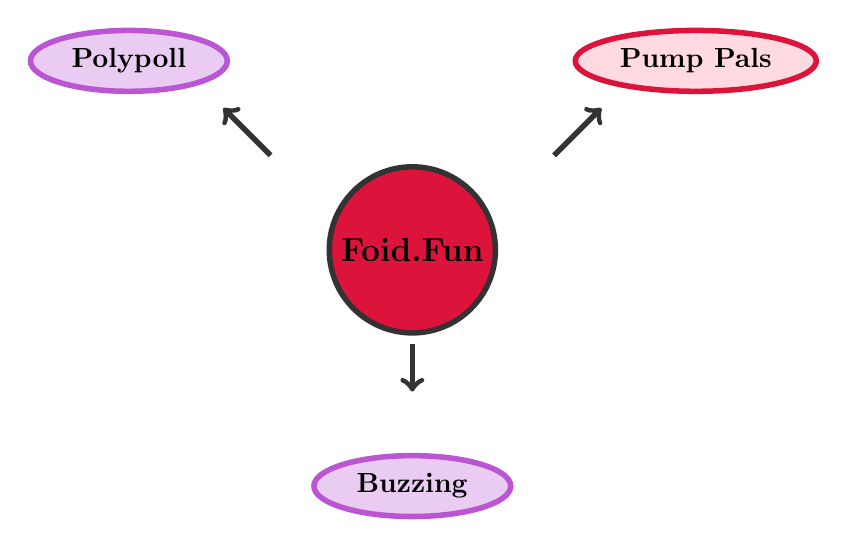
\begin{tikzpicture}[scale=1.2]
% Center node
\node[circle, fill=rebelred, draw=darkpunk, line width=2pt, minimum size=2cm] at (0,0) {
    \textbf{\large Foid.Fun}
};

% Partner nodes
\node[ellipse, fill=cuteviolet!30, draw=cuteviolet, line width=2pt, minimum width=2.5cm] at (-3,2) {\textbf{Polypoll}};
\node[ellipse, fill=punkpink!50, draw=rebelred, line width=2pt, minimum width=2.5cm] at (3,2) {\textbf{Pump Pals}};
\node[ellipse, fill=cuteviolet!30, draw=cuteviolet, line width=2pt, minimum width=2.5cm] at (0,-2.5) {\textbf{Buzzing}};

% Connections
\draw[->, line width=2pt, darkpunk] (-1.5,1) -- (-2,1.5);
\draw[->, line width=2pt, darkpunk] (1.5,1) -- (2,1.5);
\draw[->, line width=2pt, darkpunk] (0,-1) -- (0,-1.5);
\end{tikzpicture}
\end{center}
\end{frame}

% Slide 8: Foidnomics
\begin{frame}
\frametitle{Foidnomics}
\vspace{0.3cm}
\begin{center}
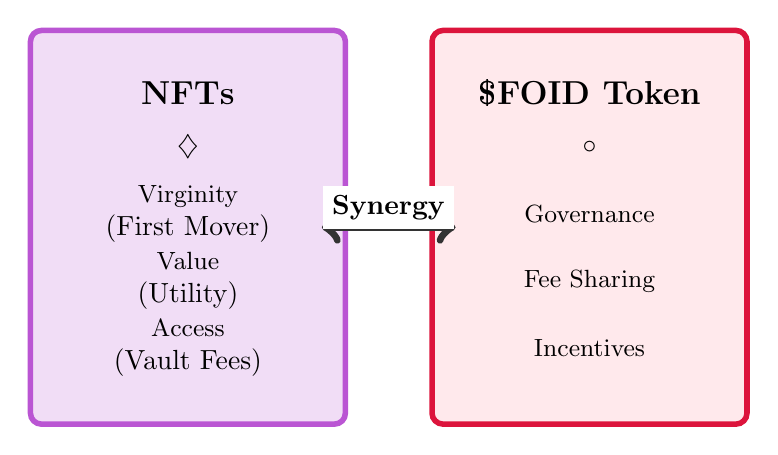
\begin{tikzpicture}[scale=0.85]
% NFT side
\node[rectangle, draw=cuteviolet, fill=cuteviolet!20, line width=2pt, rounded corners, minimum width=4cm, minimum height=5cm] at (-3,0) {};
\node at (-3,2) {\textbf{\large NFTs}};
\node at (-3,1.2) {\faImage};
\node[align=center] at (-3,0.2) {\small Virginity\\(First Mover)};
\node[align=center] at (-3,-0.8) {\small Value\\(Utility)};
\node[align=center] at (-3,-1.8) {\small Access\\(Vault Fees)};

% Token side
\node[rectangle, draw=rebelred, fill=punkpink!30, line width=2pt, rounded corners, minimum width=4cm, minimum height=5cm] at (3,0) {};
\node at (3,2) {\textbf{\large \$FOID Token}};
\node at (3,1.2) {\faCoins};
\node[align=center] at (3,0.2) {\small Governance};
\node[align=center] at (3,-0.8) {\small Fee Sharing};
\node[align=center] at (3,-1.8) {\small Incentives};

% Connection
\draw[<->, line width=3pt, darkpunk] (-1,0) -- (1,0);
\node[fill=white] at (0,0.3) {\textbf{Synergy}};
\end{tikzpicture}
\end{center}
\end{frame}

% Slide 9: Day One Launch
\begin{frame}
\frametitle{Day One Launch}
\vspace{0.5cm}
\begin{center}
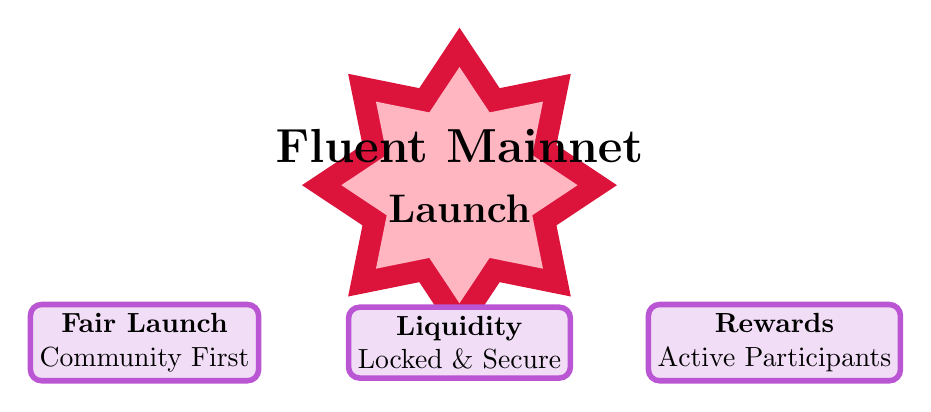
\begin{tikzpicture}
% Explosion effect for excitement
\node[star, star points=8, fill=rebelred, minimum size=4cm, inner sep=0pt] at (0,0) {};
\node[star, star points=8, fill=punkpink, minimum size=3cm, inner sep=0pt] at (0,0) {};
\node at (0,0.5) {\LARGE\textbf{Fluent Mainnet}};
\node at (0,-0.3) {\Large\textbf{Launch}};

% Tokenomics boxes
\node[rectangle, draw=cuteviolet, fill=cuteviolet!20, line width=2pt, rounded corners, align=center] at (-4,-2) {
    \textbf{Fair Launch}\\
    Community First
};
\node[rectangle, draw=cuteviolet, fill=cuteviolet!20, line width=2pt, rounded corners, align=center] at (0,-2) {
    \textbf{Liquidity}\\
    Locked \& Secure
};
\node[rectangle, draw=cuteviolet, fill=cuteviolet!20, line width=2pt, rounded corners, align=center] at (4,-2) {
    \textbf{Rewards}\\
    Active Participants
};
\end{tikzpicture}
\end{center}
\vspace{0.5cm}
\begin{center}
\Large\textcolor{rebelred}{\textit{Get Ready for Mainnet!}}
\end{center}
\end{frame}

% Slide 10: Early Contributor Rewards
\begin{frame}
\frametitle{Early Contributor Rewards}
\vspace{1cm}
\begin{itemize}
    \item[\faTwitter] \textbf{\Large Twitter Engagement Rewards}
    \begin{itemize}
        \item Earn \$FOID for quality content and community growth
    \end{itemize}
    \vspace{0.5cm}
    \item[\faTelegramPlane] \textbf{\Large Telegram Community Rewards}
    \begin{itemize}
        \item Active participation = bigger airdrop allocation
    \end{itemize}
    \vspace{0.5cm}
    \item[\faParachuteBox] \textbf{\Large Airdrop for Early Believers}
    \begin{itemize}
        \item Testnet users and community members get rewarded
    \end{itemize}
\end{itemize}
\end{frame}

% Slide 11: Consistent Stream of Innovation
\begin{frame}
\frametitle{Consistent Stream of Innovation}
\vspace{0.5cm}
\begin{center}
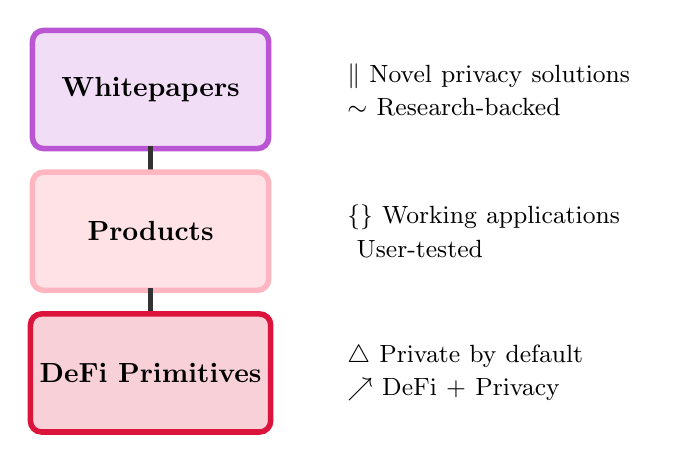
\begin{tikzpicture}[scale=0.9]
% Innovation pipeline
\node[rectangle, draw=cuteviolet, fill=cuteviolet!20, line width=2pt, rounded corners, minimum width=3cm, minimum height=1.5cm] at (0,2) {
    \textbf{Whitepapers}
};
\draw[->, line width=2pt, darkpunk] (0,1.2) -- (0,0.5);

\node[rectangle, draw=punkpink, fill=punkpink!40, line width=2pt, rounded corners, minimum width=3cm, minimum height=1.5cm] at (0,0) {
    \textbf{Products}
};
\draw[->, line width=2pt, darkpunk] (0,-0.8) -- (0,-1.5);

\node[rectangle, draw=rebelred, fill=rebelred!20, line width=2pt, rounded corners, minimum width=3cm, minimum height=1.5cm] at (0,-2) {
    \textbf{DeFi Primitives}
};

% Side annotations
\node[align=left, text width=4cm] at (5,2) {
    \small\faBook\ Novel privacy solutions\\
    \small\faPenFancy\ Research-backed
};
\node[align=left, text width=4cm] at (5,0) {
    \small\faCode\ Working applications\\
    \small\faCheckCircle\ User-tested
};
\node[align=left, text width=4cm] at (5,-2) {
    \small\faShieldAlt\ Private by default\\
    \small\faChartLine\ DeFi + Privacy
};
\end{tikzpicture}
\end{center}
\end{frame}

% Slide 12: Doxxed Devs
\begin{frame}
\frametitle{Doxxed Devs}
\vspace{0.3cm}
\begin{center}
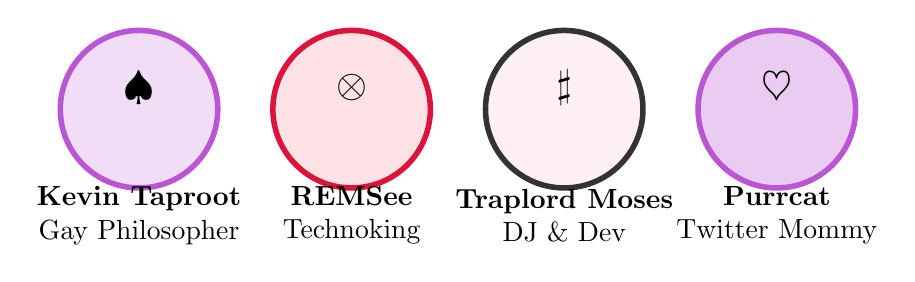
\begin{tikzpicture}[scale=0.9]
% Kevin
\node[circle, draw=cuteviolet, fill=cuteviolet!20, line width=2pt, minimum size=2cm] at (-4,1.5) {};
\node at (-4,1.8) {\Large\faCrown};
\node[align=center] at (-4,0) {\textbf{Kevin Taproot}\\Gay Philosopher};

% REMSee
\node[circle, draw=rebelred, fill=punkpink!40, line width=2pt, minimum size=2cm] at (-1,1.5) {};
\node at (-1,1.8) {\Large\faCog};
\node[align=center] at (-1,0) {\textbf{REMSee}\\Technoking};

% Traplord Moses
\node[circle, draw=darkpunk, fill=punkpink!20, line width=2pt, minimum size=2cm] at (2,1.5) {};
\node at (2,1.8) {\Large\faMusic};
\node[align=center] at (2,0) {\textbf{Traplord Moses}\\DJ \& Dev};

% Purrcat
\node[circle, draw=cuteviolet, fill=cuteviolet!30, line width=2pt, minimum size=2cm] at (5,1.5) {};
\node at (5,1.8) {\Large\faCat};
\node[align=center] at (5,0) {\textbf{Purrcat}\\Twitter Mommy};
\end{tikzpicture}
\end{center}
\vspace{0.5cm}
\begin{center}
\large\textcolor{darkpunk}{\textit{Real people, real commitment}}
\end{center}
\end{frame}

% Slide 13: Unstoppable Community Development
\begin{frame}
\frametitle{Unstoppable Community Development}
\vspace{0.5cm}
\begin{center}
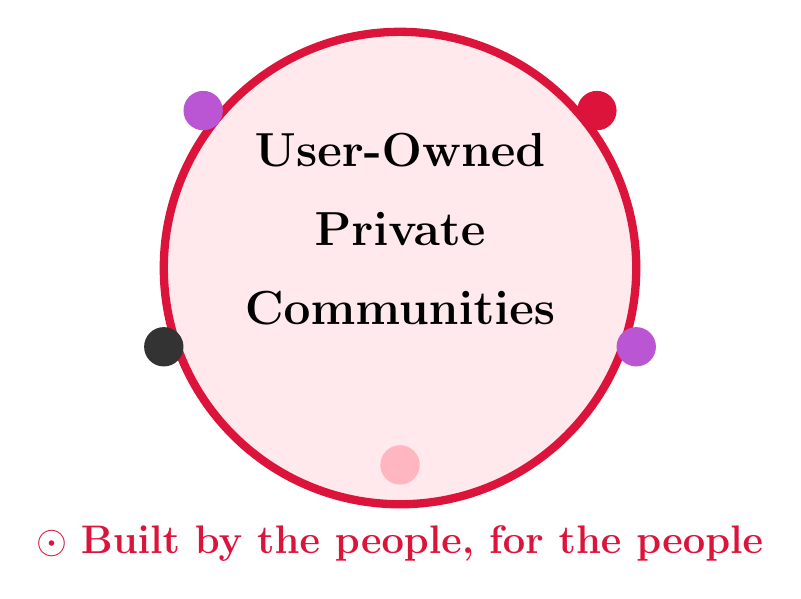
\begin{tikzpicture}
% Community circle
\node[circle, draw=rebelred, fill=punkpink!30, line width=3pt, minimum size=6cm] at (0,0) {};
\node at (0,1.5) {\LARGE\textbf{User-Owned}};
\node at (0,0.5) {\LARGE\textbf{Private}};
\node at (0,-0.5) {\LARGE\textbf{Communities}};

% Connecting elements around
\node[circle, fill=cuteviolet, minimum size=0.5cm] at (-2.5,2) {};
\node[circle, fill=rebelred, minimum size=0.5cm] at (2.5,2) {};
\node[circle, fill=darkpunk, minimum size=0.5cm] at (-3,-1) {};
\node[circle, fill=cuteviolet, minimum size=0.5cm] at (3,-1) {};
\node[circle, fill=punkpink, minimum size=0.5cm] at (0,-2.5) {};

\node at (0,-3.5) {\Large\textcolor{rebelred}{\faUsers\ \textbf{Built by the people, for the people}}};
\end{tikzpicture}
\end{center}
\end{frame}

% Slide 14: Conclusion
\begin{frame}[plain]
\begin{center}
\vspace{1.5cm}
{\Huge\textbf{\textcolor{rebelred}{Privacy \& Memes}}}

\vspace{0.8cm}

{\LARGE\textcolor{cuteviolet}{on}}

\vspace{0.8cm}

{\Huge\textbf{\textcolor{darkpunk}{Fluent}}}

\vspace{1.5cm}


\begin{tikzpicture}
\node[rectangle, draw=rebelred, fill=punkpink!40, line width=3pt, rounded corners, minimum width=8cm, minimum height=1.5cm] at (0,0) {
    \Large\textbf{Foid.Fun: Where Privacy Meets Culture}
};
\end{tikzpicture}
\end{center}
\end{frame}

\end{document}
